\documentclass[tikz, border=10pt]{standalone}

\usetikzlibrary{arrows}

\begin{document}
	
	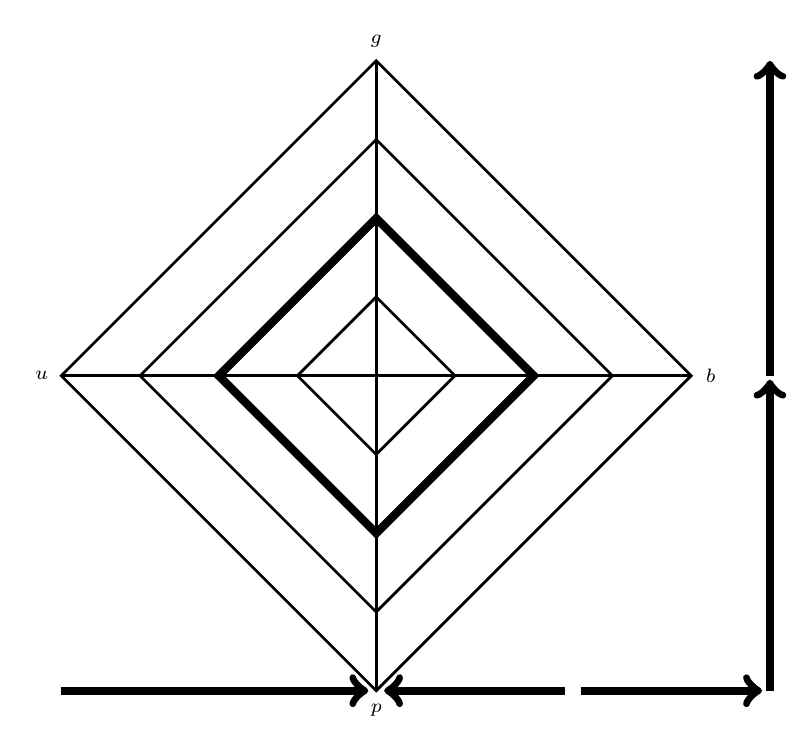
\begin{tikzpicture}[line width=1pt]
		\draw (0, 4) -- (4, 0) -- (8, 4) -- (4, 8) -- cycle;
		\draw (4, 1) -- (1, 4) -- (4, 7) -- (7, 4) -- cycle;
		\draw[line width=3pt] (4, 6) -- (2, 4) -- (4, 2) -- (6, 4) -- cycle;
		\draw (4, 5) -- (3, 4) -- (4, 3) -- (5, 4) -- cycle;
		
		\draw (4, 8) -- (4, 0);
		\draw (0, 4) -- (8, 4);
		
		\draw[->, line width=3pt] (9, 4) -- (9, 8);
		\draw[->, line width=3pt] (9, 0) -- (9, 3.95);
		
		\draw[->, line width=3pt] (6.6, 0) -- (8.9, 0);
		\draw[<-, line width=3pt] (4.1, 0) -- (6.4, 0);
		
		\draw[->, line width=3pt] (0, 0) -- (3.9, 0);

	\begin{scriptsize}
		\draw (-0.25, 4) node {$u$};
		\draw (4, 8.25) node {$g$};
		\draw (8.25, 4) node {$b$};
		\draw (4, -0.25) node {$p$};
	\end{scriptsize}

\end{tikzpicture}
\end{document}